%dispTree -ll -gg -w -s 85 -t

\documentclass{beamer}
%\usetheme{Madrid}
%\usetheme{Boadilla}
%\usetheme{default}
%\usetheme{Warsaw}
%\usetheme{Bergen}
%\usetheme{Frankfurt}
\usetheme{Darmstadt}

%\usecolortheme{seahorse}
%\usecolortheme{beaver}
\usecolortheme[named=orange]{structure}

\setbeamertemplate{footline}[page number]
%\setbeamercovered{transparent}
\setbeamercovered{invisible}
\setbeamertemplate{navigation symbols}{}

\usepackage{multimedia}
\usepackage{graphicx}
\usepackage[utf8]{inputenc}
%\usepackage[T1]{fontenc}
\usepackage[frenchb]{babel} 
\usepackage[all]{xy}
\usepackage{multirow}
\usepackage{lmodern}
\usepackage{subfigure}
\usepackage{ulem}
\usepackage{hyperref}
\usepackage{pifont}

%% --------------

\title[Soutenance AI]{Debriefing Année Internationale}
\author{L\'eo B\textsc{audouin}}
\institute[LAAS-CNRS]
{
Japon - Replanification en temps réel pour les robots humanoïdes\\NZ - Controle en force d'un bras anthropomorphe
\\
\medskip
{\emph{leo.baudouin@ifma.fr}}
}
\date{20 janvier 2012}

%% --------------

\begin{document}

\begin{frame}
\titlepage
\end{frame}

\begin{frame}{Japon}
\tableofcontents
\end{frame}

\section{Japon}
\subsection{Tsukuba}
\begin{frame}
%	\begin{block}{\begin{center}Tsukuba\end{center}}
	\begin{center}
	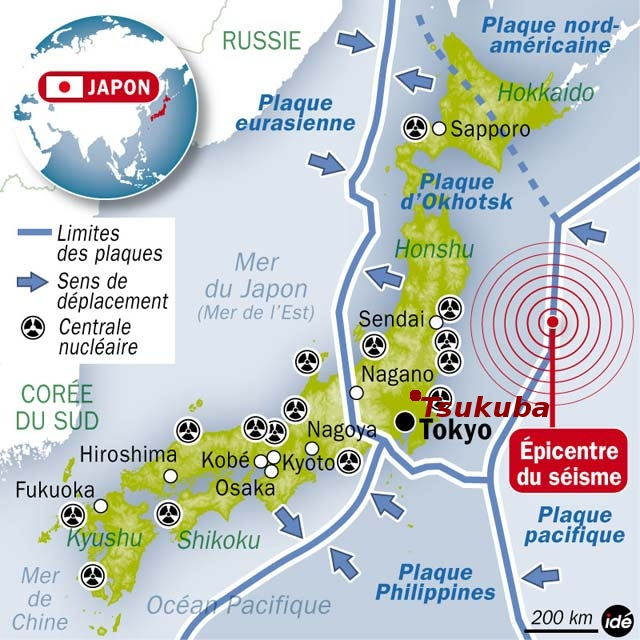
\includegraphics[width=0.7\linewidth]{images/carte1}
	\end{center}
%	\end{block}
\end{frame}

\subsection{Visites}
\begin{frame}
\begin{center}
Du 14 Février au 13 Mars 2011\\
Tsukuba \ding{224} Tsuchiura \ding{224} T\=oky\=o
\end{center}
 \begin{figure}
      \subfigure[\small Akihabara]{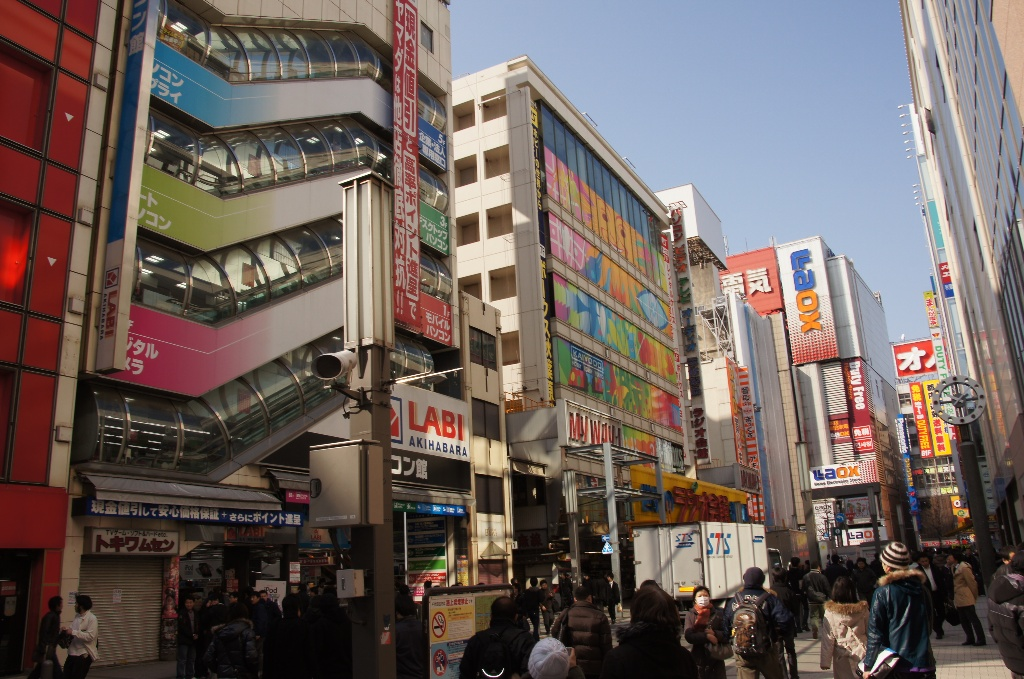
\includegraphics[width=0.5\linewidth]{./images/DSC00887}}~
      \subfigure[\small Shibuya]{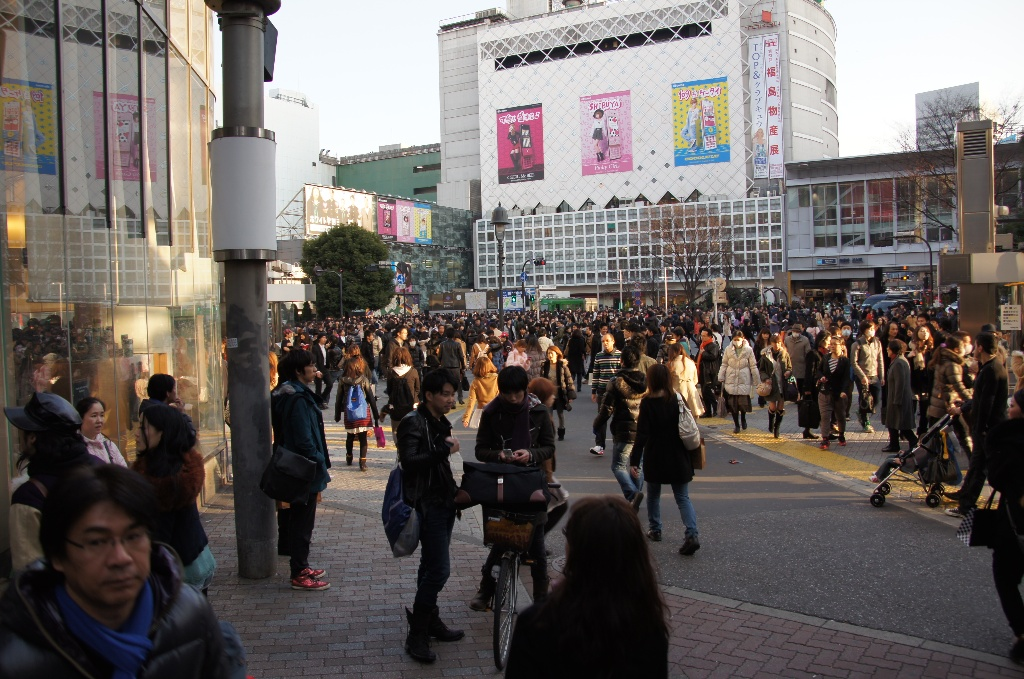
\includegraphics[width=0.5\linewidth]{./images/DSC00975}}
    \end{figure}
    
\end{frame}

\subsection{Laboratoire}
\begin{frame}{AIST/JRL - LAAS}
\begin{tabular}{c | c}
\begin{minipage}{0.5\linewidth}
\begin{center}

\includegraphics[width=0.5\linewidth]{./images/AIST}\\
\vspace{5mm}
{\huge AIST/JRL}
\end{center}
\begin{itemize}
\item Laboratoire Franco-Japonais
\item 15 personnes environ
\item Un HRP-2
\end{itemize}
\end{minipage}
&
\begin{minipage}{0.5\linewidth}
\begin{center}
\vspace{5mm}

\includegraphics[width=0.5\linewidth]{./images/LAAS}\\
\vspace{5mm}
{\huge LAAS}
\end{center}
\begin{itemize}
\item Groupe Gepetto
\item 15 personnes environ
\item Un HRP-2
\end{itemize}
\end{minipage}
\end{tabular}
\end{frame}

\setcounter{subfigure}{0}

\section{Etat de l'art}
\subsection*{Littérature scientifique}
\begin{frame}
  \center Replanification en robotique humanoïde
  \begin{figure}
    \subfigure[A\textsc{simo} navigant dans un environnement 2D mobile.]{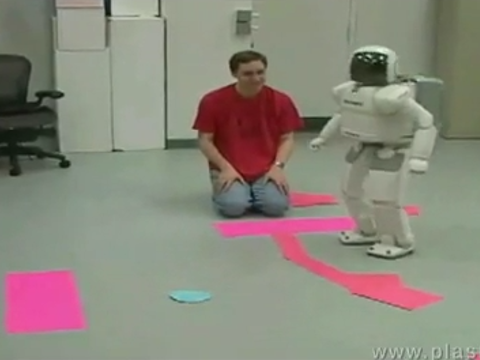
\includegraphics[width=6cm]{./images/Asimo.png}}~
    \subfigure[Pas admissibles pour la planification.]{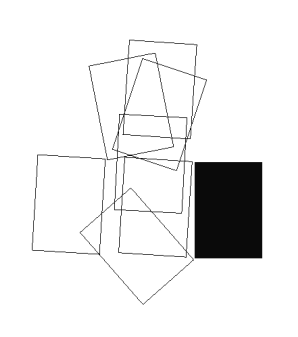
\includegraphics[width=4cm]{./images/FewSteps.png}}\\
  \end{figure}

  \begin{small}
    \emph{Footstep planning for the Honda ASIMO Humanoid}\\
    J. Chestnutt, M. Lau, G. Cheung, J. Kuffner, J. Hodgins, and T. Kanade.\\
    \textit{In IEEE/RAS Int.Conf. on Robotics and Automation}, 2005
  \end{small}

\end{frame}

%\begin{frame}
% \center Replanification en robotique humanoïde
%  \begin{figure}
%    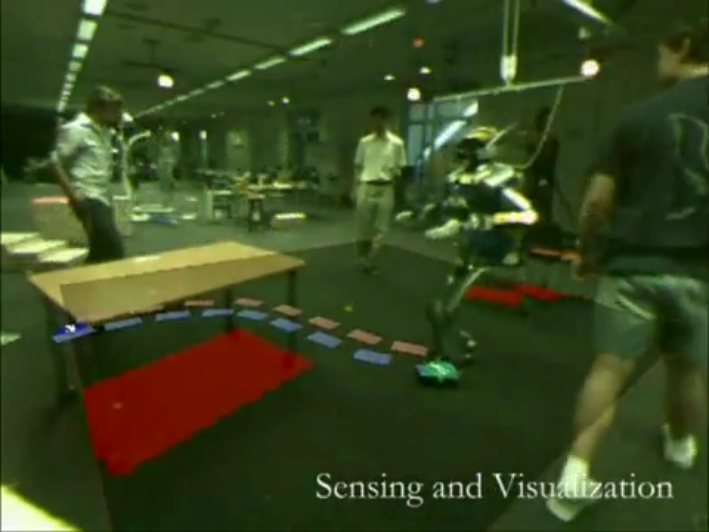
\includegraphics[width=6cm]{./images/Hrp2.png}\\
%    Projections en rouge des obstacles 3D.
%  \end{figure}
%
%  \begin{small}
%    \emph{Motion Planning for Humanoid Robots}.\\
%    Chestnutt, K. Harada, E. Yoshida, and Y. Kazuhito.\\
%    Chapter Navigation and gait planning, pages 1-28. Springer-Verlag, 2010.
%  \end{small}
%
%\end{frame}

\begin{frame}
  \begin{center}
    Planification dans un environnement contraint\\
    \vspace{3mm}
    %\movie{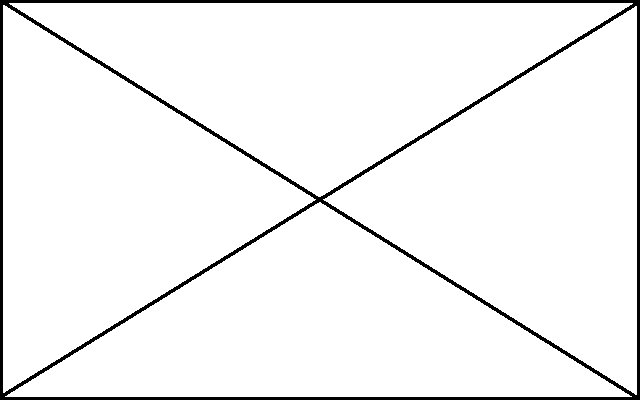
\includegraphics[width=7cm]{./images/vide.jpg}}{./videos/SteppingOverObstaclesFastPlanning.avi}\\
    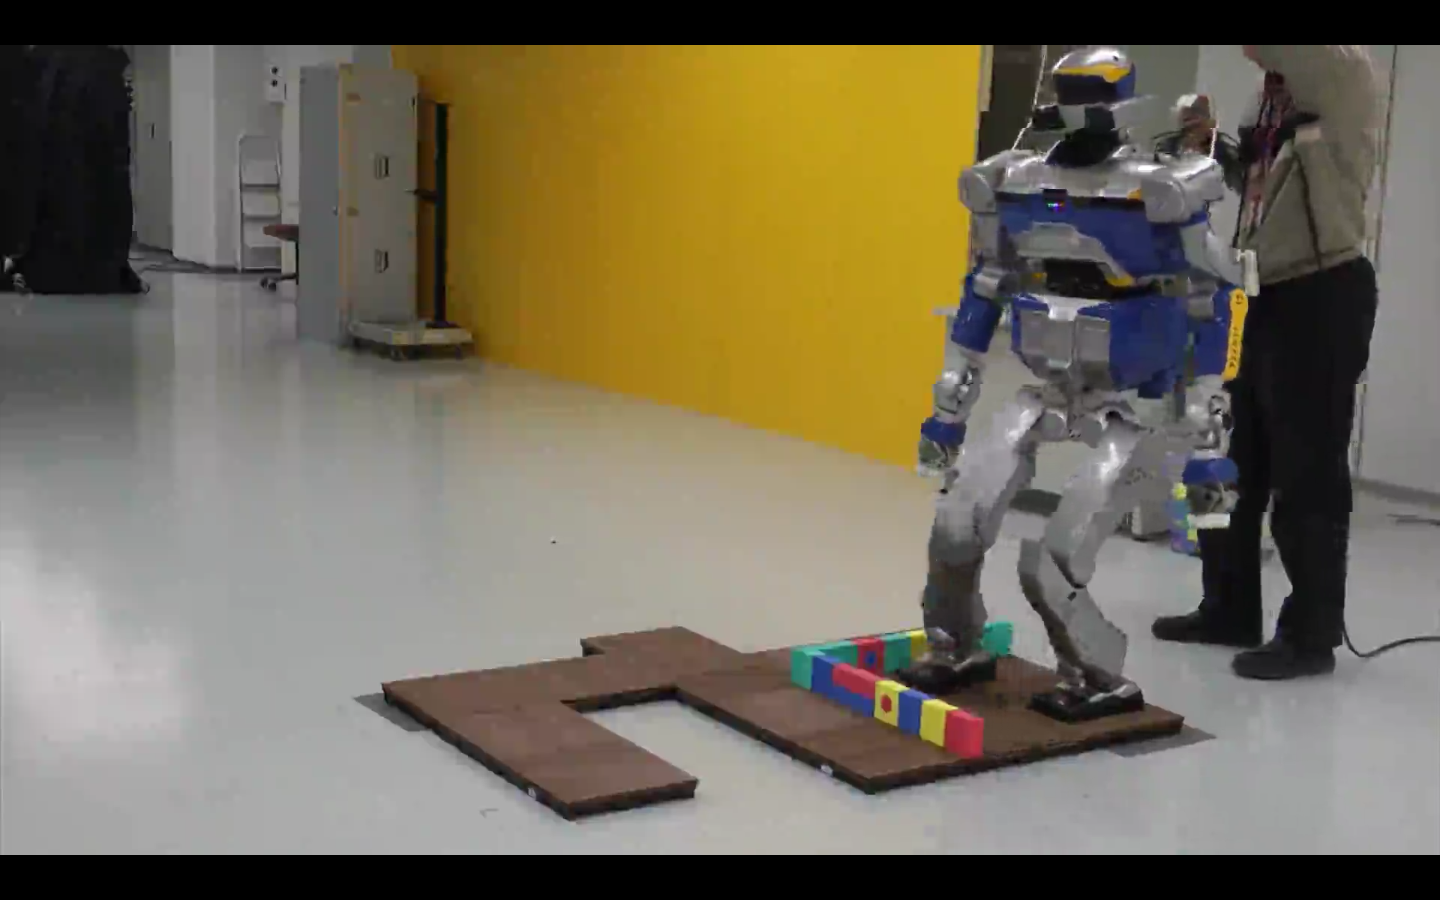
\includegraphics[width=7cm]{./images/img1}\\
  \end{center}

  \begin{center}
    \begin{small}
      \emph{Fast humanoid robot collision-free footstep planning using\\ swept volume approximations}\\
      N. Perrin, O. Stasse, L. Baudouin, F. Lamiraux, and E. Yoshida.\\
      \textit{IEEE Transactions on Robotics}, 2011.
    \end{small}
  \end{center}
\end{frame}

\section{Planification}

%\subsection{Demi-pas}
%\begin{frame}
%  \begin{center}
%    Notion de séquence de demi-pas quasi-statiques.
%    \begin{figure}
%      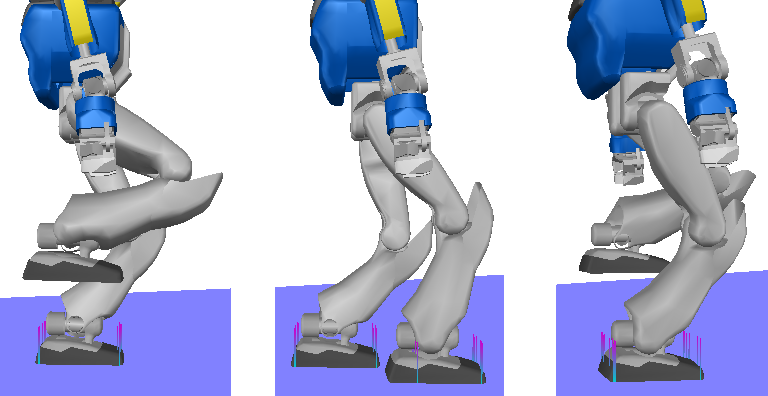
\includegraphics[width=8cm]{./images/HalfStep.png}\\
%    \end{figure}
%   \end{center}
%  Un pas complet se fait en 4 phases :
%  \begin{small}
%    \begin{itemize}
%    \item Phase stable de simple support
%    \item Phase de vol
%    \item Phase stable de double support
%    \item Phase de vol
%    %\item Phase stable de simple support
%    \end{itemize}
%    \end{small}
%\end{frame}

% --------------

\subsection{Rapidly-exploring Random Trees - RRT}

\begin{frame}
  \center Recherche de chemin : Rapidly-exploring Random Trees (RRT)
  \begin{columns}
    \begin{column}{7cm}
      %\begin{columns}{1cm}
      \begin{itemize}
      \item Avantages :
        \begin{itemize}
        \item Rapidité des itérations
        \item Couverture de l'espace
        \item Evite les miminums locaux
        \item Nombre de pas admissibles important
        \end{itemize}
        \vspace{3mm}
      \item Inconvénients :
        \begin{itemize}
        \item Trajectoires non-optimales
        \item Imprévisible
        \end{itemize}
      \end{itemize}
    \end{column}

    \begin{column}{4cm}
      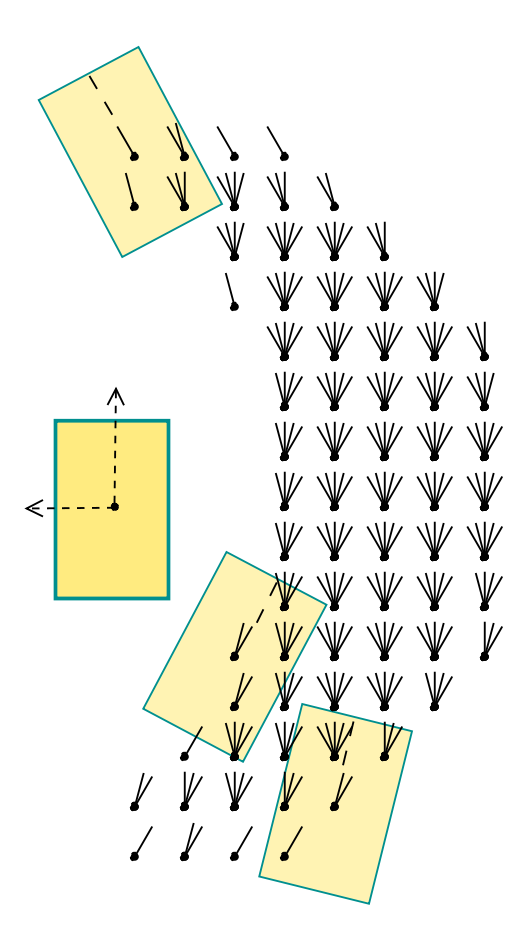
\includegraphics[width=3cm]{./images/grid_simple.png}
    \end{column}
  \end{columns}

  \vspace{5mm}
  Exemple : Vitesse de création d'un arbre RRT avec des obstacles.
\end{frame}

\begin{frame}

  \begin{figure}
    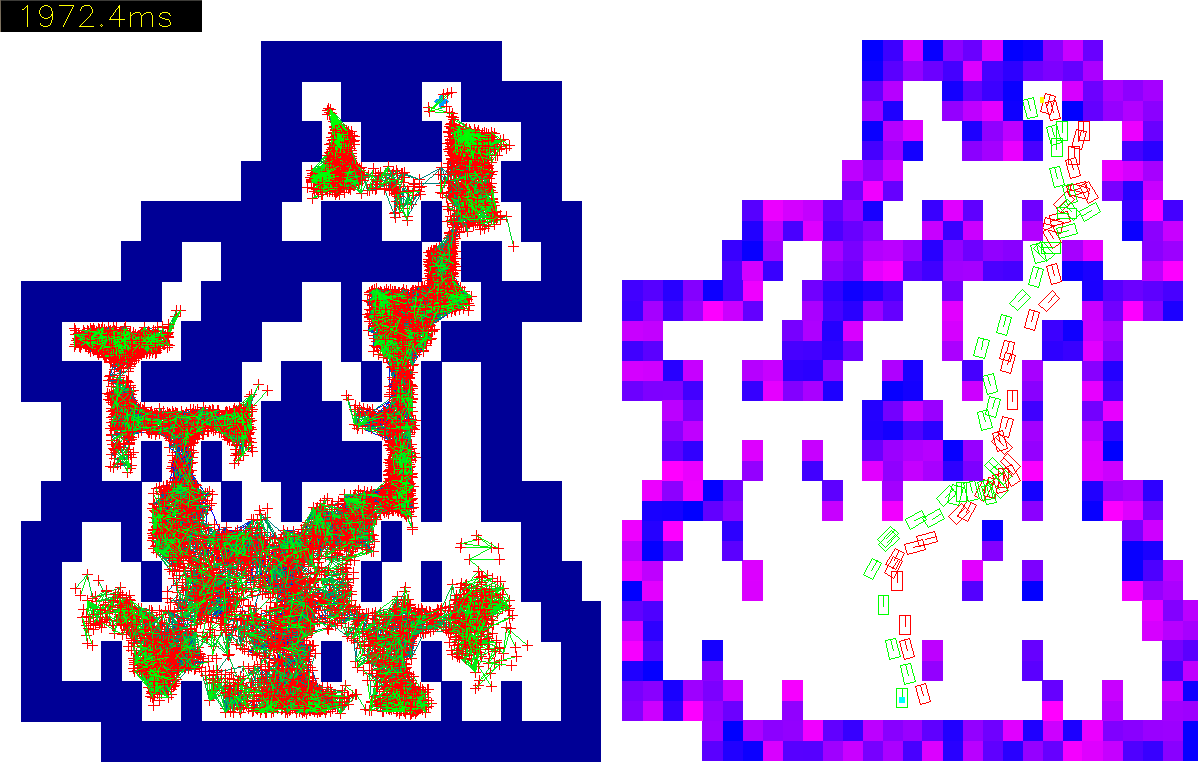
\includegraphics[width=11cm]{./images/RRT.png}
  \end{figure}
\end{frame}

\subsection{Volumes balayés}

\begin{frame}
  \begin{center}
    Détection de collision : Proximity Query Package - PQP
    \begin{figure}
      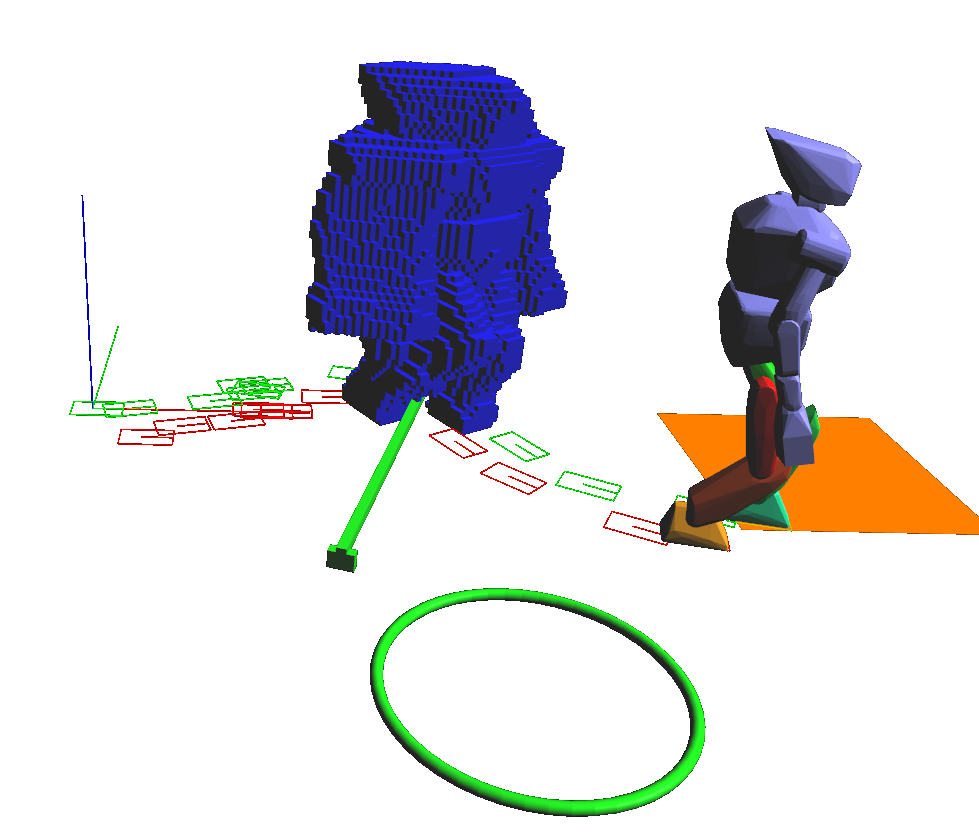
\includegraphics[width=7cm]{./images/SV.png}
      \caption{Volume balayé sur un pas}
    \end{figure}
    %Utilisation de PQP avec des volumes balayés.
  \end{center}
\end{frame}

%\begin{frame}
%  \center Approximation des volumes balayés
%  \begin{tiny}
%    \begin{figure}
%      \subfigure[\tiny{Original - 1.687.596}]{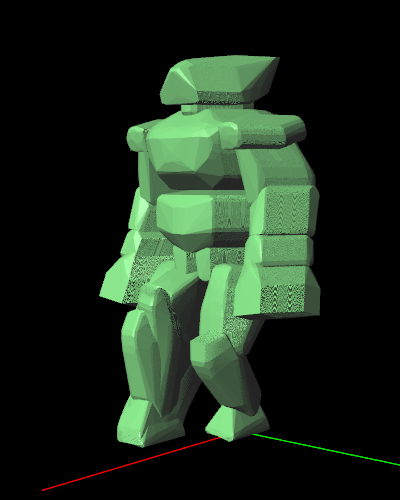
\includegraphics[width=2.5cm]{./images/SV_original.png}}~
%      \subfigure[\tiny{5mm - 508.120}]{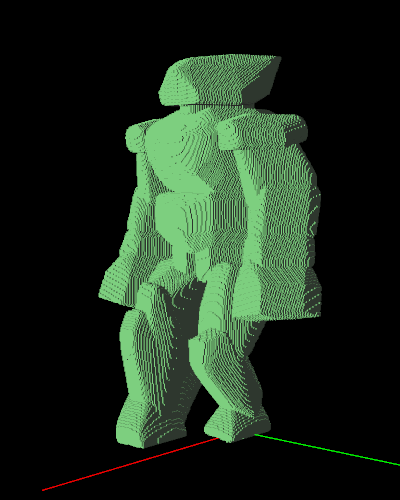
\includegraphics[width=2.5cm]{./images/SV_5mm.png}}~
%      \subfigure[\tiny{10mm - 125.772}]{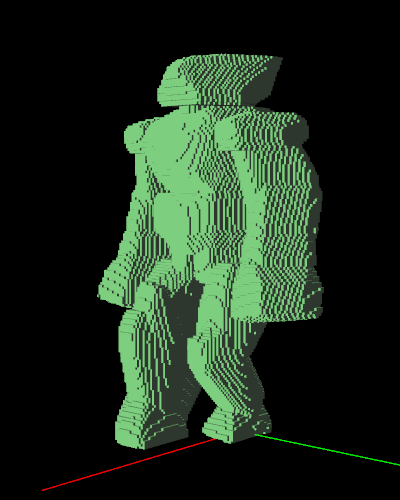
\includegraphics[width=2.5cm]{./images/SV_10mm.png}}
%    \end{figure}
%    \vspace{-7mm}
%    \begin{figure}
%      \subfigure[\tiny{25mm - 19.524}]{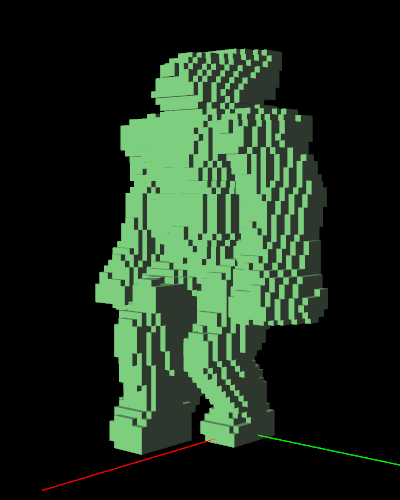
\includegraphics[width=2.5cm]{./images/SV_25mm.png}}~
%      \subfigure[\tiny{50mm - 4.596}]{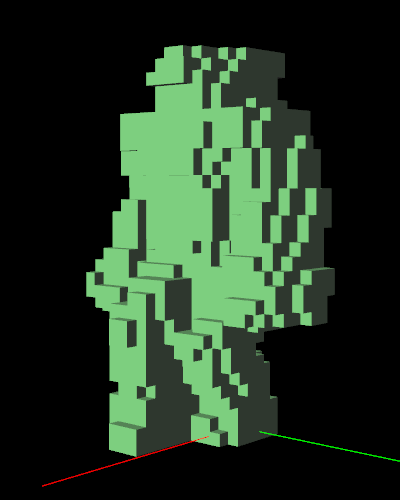
\includegraphics[width=2.5cm]{./images/SV_50mm.png}}~
%      \subfigure[\tiny{100mm - 1.144}]{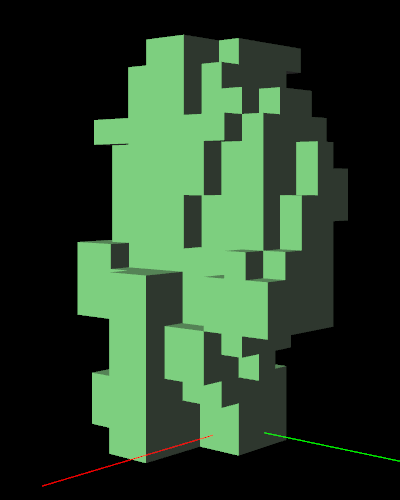
\includegraphics[width=2.5cm]{./images/SV_100mm.png}}
%    \end{figure}
%  \end{tiny}
%\end{frame}

%\subsection{Lissage de trajectoire}
%\begin{frame}
%  \begin{center} 
%    Accélération des trajectoires
%    \begin{figure}
%      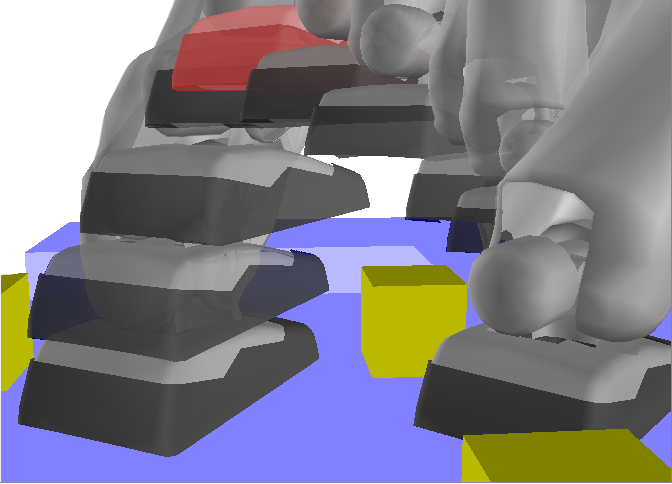
\includegraphics[width=5cm]{./images/smoothing_before.png}~
%      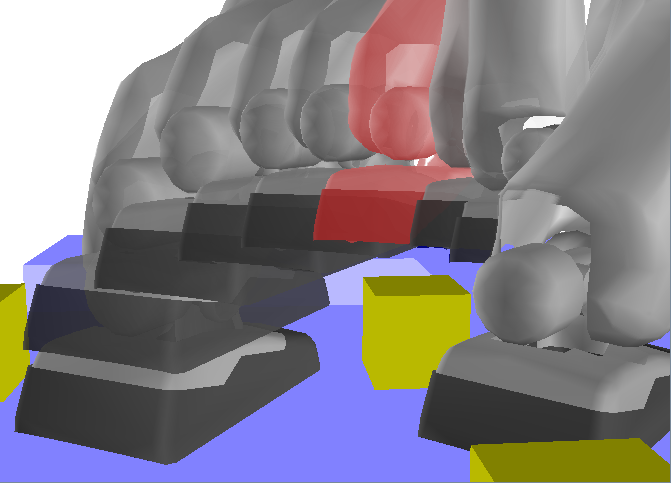
\includegraphics[width=5cm]{./images/smoothing_after.png}
%    \end{figure}
%    
%    Suppression de la phase de double support\\
%    Réduction au mieux de la phase de simple support
%  \end{center}
%\end{frame}

% --------------

%\section{Expériences}
%\subsection{Matériel}
%\begin{frame}
%  \begin{figure}
%    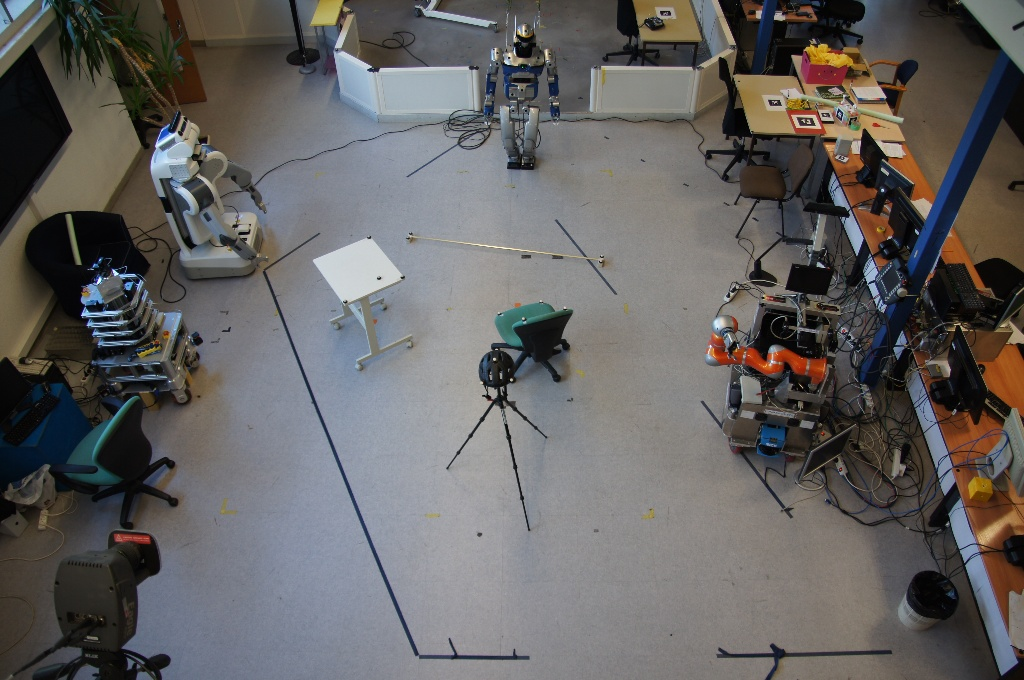
\includegraphics[width=9cm]{./images/grande_salle.jpg}\\
%    Grande salle d'expérience robotique du LAAS.
%  \end{figure}
%\end{frame}

%\subsection*{Motion capture}
%\begin{frame}
%  \center Détection des différents objets avec la \textit{motion capture}.\\
%   \begin{figure}
%    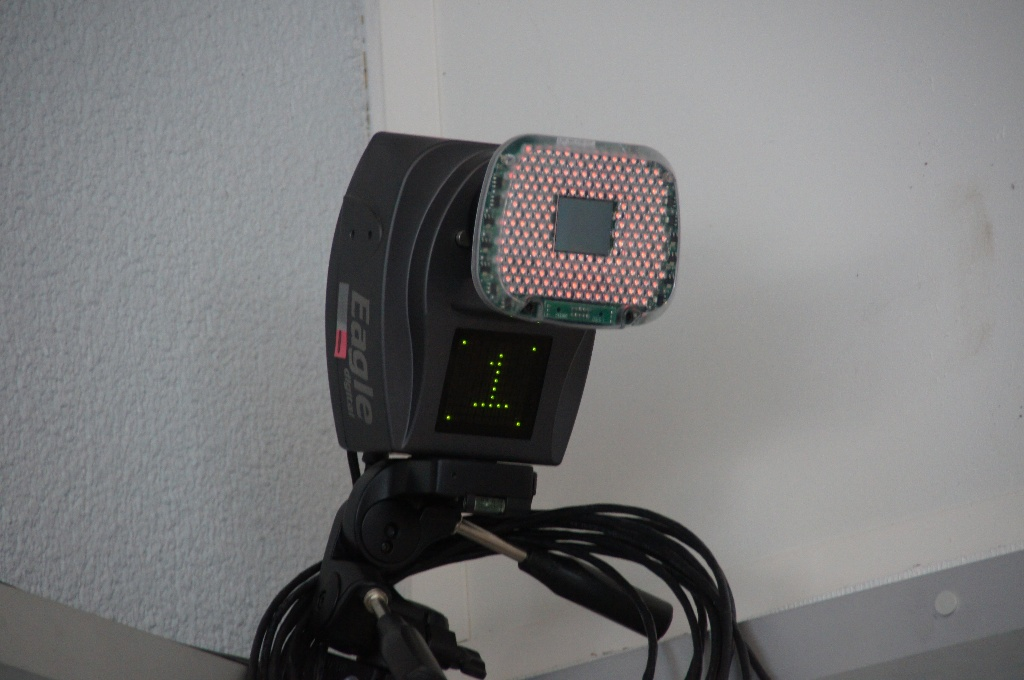
\includegraphics[width=4.5cm]{./images/IR.jpg}~
%    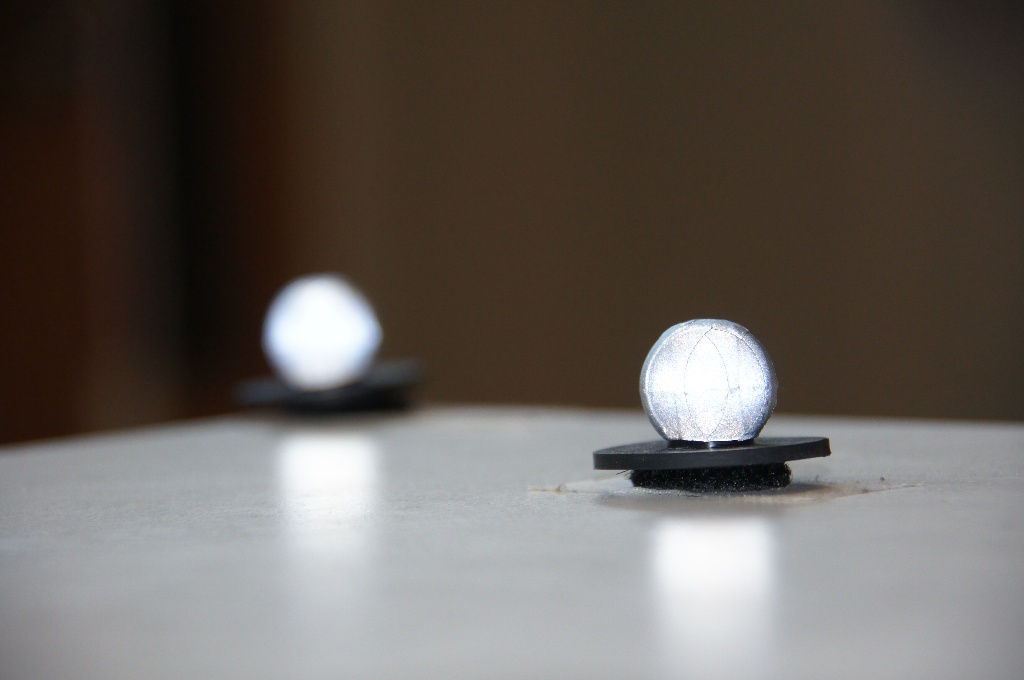
\includegraphics[width=4.5cm]{./images/marker_flash.jpg}
%  \end{figure}
%  \vspace{-5mm}
%  \begin{figure}
%    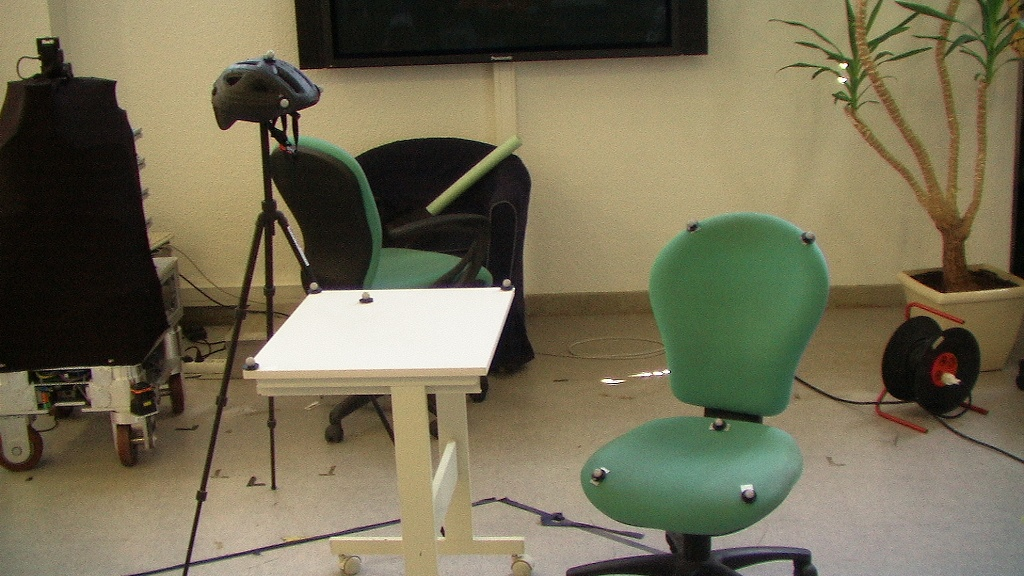
\includegraphics[width=5cm]{./images/mocap_real.jpg}~
%    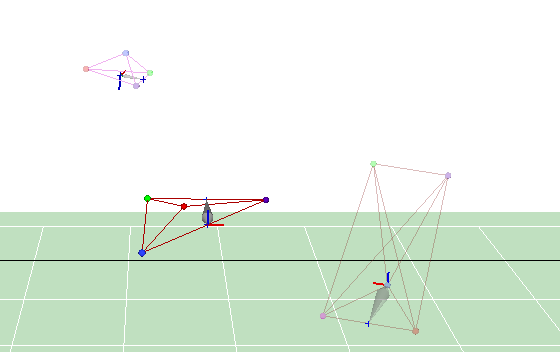
\includegraphics[width=5cm]{./images/mocap.png}
%  \end{figure}
%\end{frame}

\subsection{Résultats}
\begin{frame}
  \begin{figure}
    %\movie{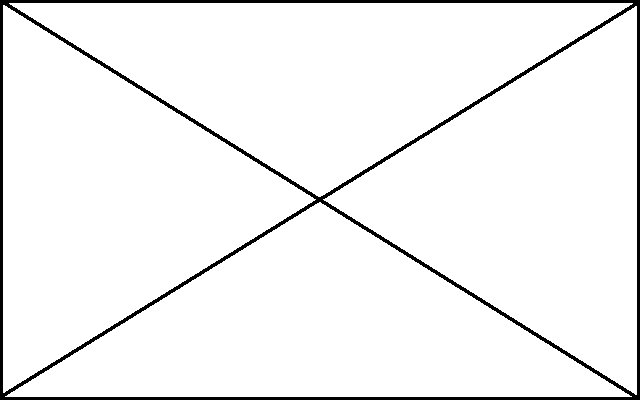
\includegraphics[width=9cm]{./images/vide.jpg}}{./videos/humanoids11-lbaudouin.avi}\\
	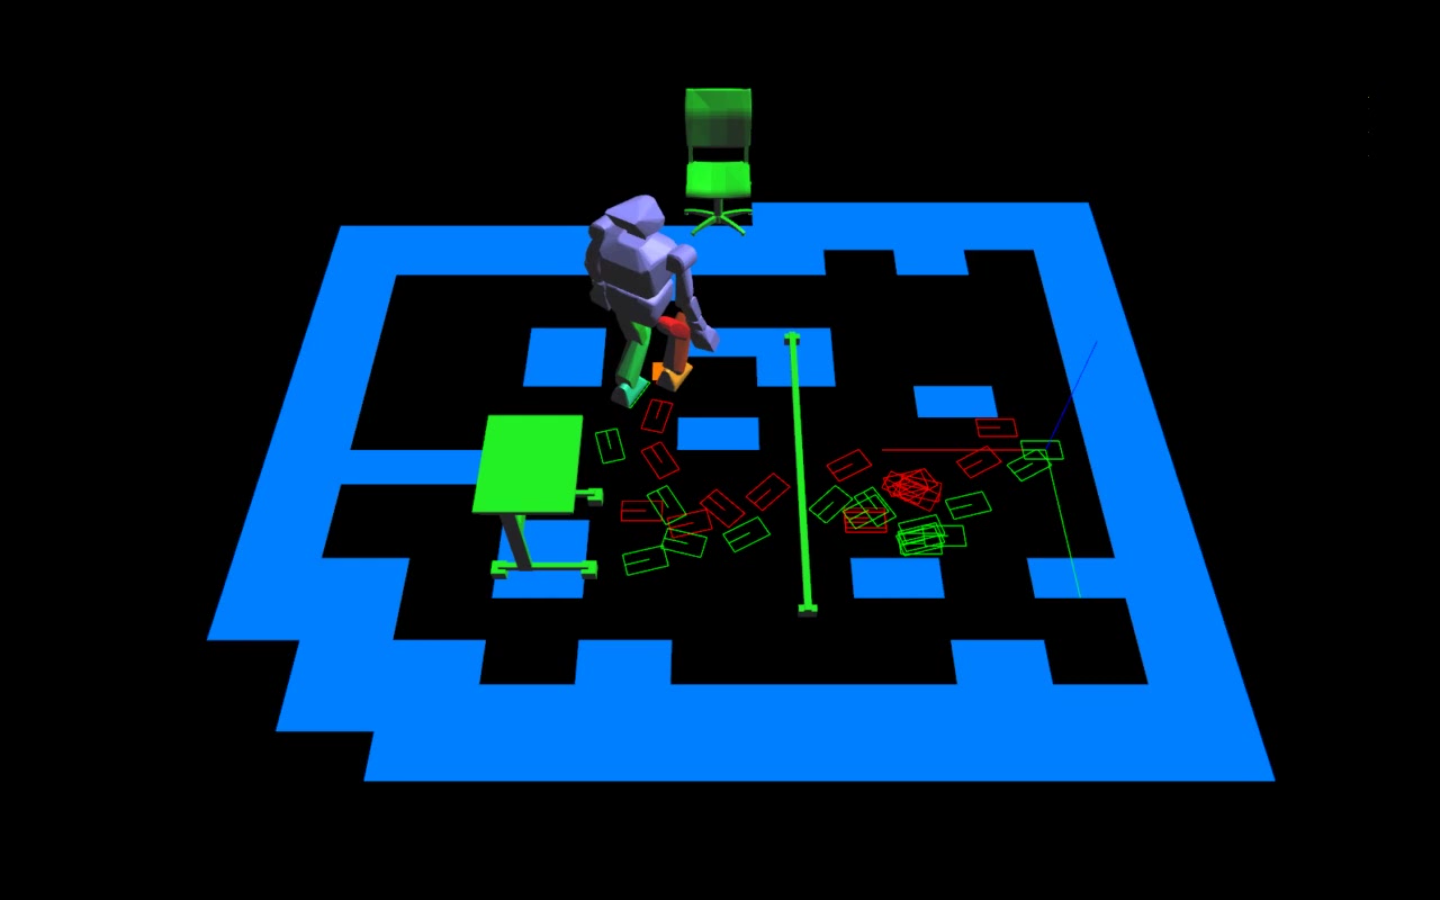
\includegraphics[width=9cm]{./images/img2}\\    
    Vidéo publiée à Humanoids'11
   \end{figure}
 \end{frame}

\section{Conclusion}
\subsection{Résultats}

\begin{frame}
  \begin{itemize}
  \item  Performances :
    \begin{itemize}
    \item Vitesse de planification
    \item Enjambement d'obstacles
    \item Replanification
    \end{itemize}
    \vspace{3mm}
  \item Points restants à améliorer :
    \begin{itemize}
    \item Vitesse de marche du robot
    \item Précision sur la position du pied
    \item Rendre le robot complètement autonome
    \end{itemize}
  \end{itemize}
\end{frame}

% --------------

\subsection{Publications}
\begin{frame}
\begin{itemize}
\item International
  \begin{itemize}
    \item Humanoids 2011 :\\
\textbf{L. Baudouin}, N. Perrin, O. Stasse, T. Moulard, E. Yoshida, and F. Lamiraux. \emph{Real-time Replanning Using 3D Environment for Humanoid Robot}.
In \textit{IEEE Int. Conf. on Humanoid Robotics (Humanoids’11)}, 2011.

    \item Transactions on Robotics 2011 :\\
N. Perrin, O. Stasse, \textbf{L. Baudouin}, F. Lamiraux, and E. Yoshida. \emph{Fast Humanoid Robot Collision-Free Footstep Planning Using Swept Volume Approximations}. \textit{IEEE Transactions on Robotics}, 2011. conditionnally accepted.
\end{itemize}
\item National
\begin{itemize}
    \item Robotics Society of Japan 2011 :\\
\textbf{L. Baudouin}, N. Perrin, O. Stasse, T. Moulard, E. Yoshida, and F. Lamiraux. \emph{Real-time Replanning Using 3D Environment for Humanoid Robot}.
In \textit{RSJ11}, 2011.
      \end{itemize}
  \end{itemize}
\end{frame}

%\subsection{Conclusion}
%\begin{frame}
%\end{frame}

%\subsection*{Conclusion Générale}
%\begin{frame}
%  \begin{itemize}
%  \item Travaux de recherche
%    \begin{itemize}
%    \item Intérêts
%    \item Difficultés
%    \item Publications
%   \end{itemize}
%  \item Programmation
%    \begin{itemize}
%    \item Packaging
%    \item Langages
%    \end{itemize}
%  \item Poursuite du projet
%    \begin{itemize}
%    \item Applications
%    \item Limites
%    \end{itemize}
%  \end{itemize}
%\end{frame}


%% -------------

\setcounter{page}{23}

\end{document}  
